\documentclass{standalone}
\usepackage{pgfplots}
\begin{document}
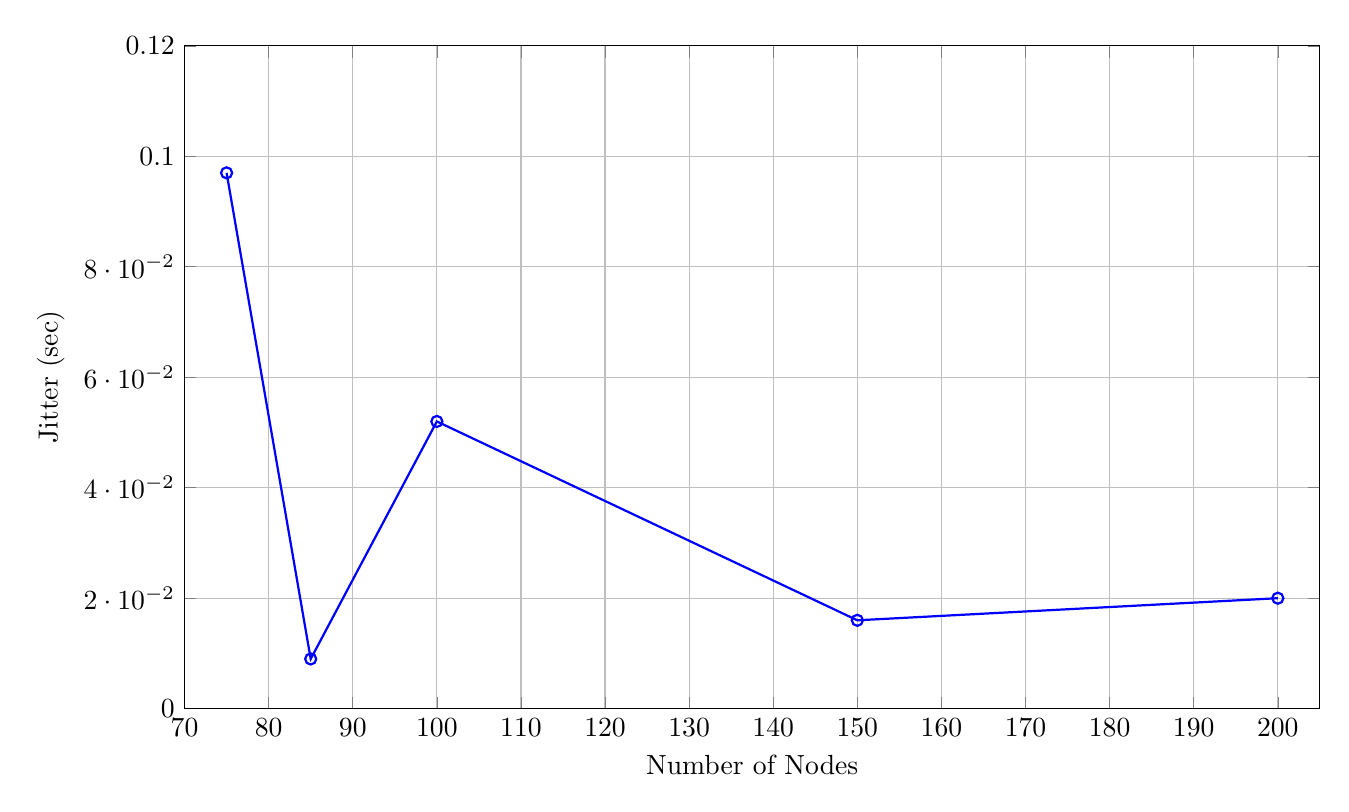
\begin{tikzpicture}
\begin{axis}[
width=16cm,height=10cm,
xlabel={Number of Nodes},
ylabel={Jitter (sec)},
xmin=70,xmax=205,
ymin=0.0,ymax=0.12,
grid=major
]
\addplot+[mark=o,thick] coordinates {
(75,0.097)(85,0.009)(100,0.052)(150,0.016)(200,0.020)
};
\end{axis}
\end{tikzpicture}
\end{document}